\chapter{Performance evaluation of Cached}\label{ch:cached-evaluation}

\begin{flushright}
	\textit{"There are three kinds of lies:\\
		lies, damned lies, \\
		and \sout{statistics} benchmarks."}	\\

	Mark Twain (modernized)
\end{flushright}

It may seem as an ironic statement, considering that we are about to provide 
benchmark results for cached, but it actually is a very valid one. What Mr.  
Twain tries to say here
\footnote{
	a phrase usually not heard in programming contexts...
}
is that the presentation of partials facts for something can be used to 
fabricate a plausible truth for it. In science's case, it so often happens that 
promising results for an experiment can seem more important to the researcher's 
eye than negative ones due to positive reinforcement.

In out case, we will try not to merely smear the next pages with diagrams but 
first explain the benchmarking methodology behind them.

The skeleton of this chapter is the following: Section \ref{sec:perf-meth} 
explains the methodology behind our measurements. Section \ref{sec:perf-plot} 
presents the results of the benchmarks that we have done and provides in-depth 
explanations about each of them. Finally, Section ? is undefined.

\section{Benchmark methodology}

The benchmarks that have been executed and whose results are presented in this 
chapter, will be split in two categories, both of which have their own distinct 
goals:

The first category is the comparison between using cached on top of the sosd 
(sosd has been discussed here ?) and using solely the sosd. The category's goal 
is to "defend" one of the core thesis arguments, that tiering is a key element 
that will improve the performance of Archipelago. 

In order to compare effectively the performance of cached and sosd, we must 
consider the following: 

\begin{enumerate}[i]
	\item The comparisons of two peers are should not aim to test the all 
		the implementation settings but focus on what is the best 
		performance that these peers can achieve.
	\item Both peers must be tested with the under the same, reasonable 
		workload.
	\item The workload must be reasonable i.e can be encountered in 
		production environments and test


We must also tackle one more problem, that is which results to show. Our 
implementation has many different aspects which deserve their own benchmarks and 
these are

\begin{enumerate}
	\item Bucket size
	\item IOdepth
	\item Cache size
	\item Max cached objects
	\item Write policy
	\item ...
\end{enumerate}

For this reason, we have to distinguish between which are more important 
payloads and which not. Important payloads are considered payloads that are met 
in production environments. The most troublesome payload of production 
environments is by far the stampede of 4k random writes and this is the one that 
we will view first.

\begin{figure}[hb]
	\centering
	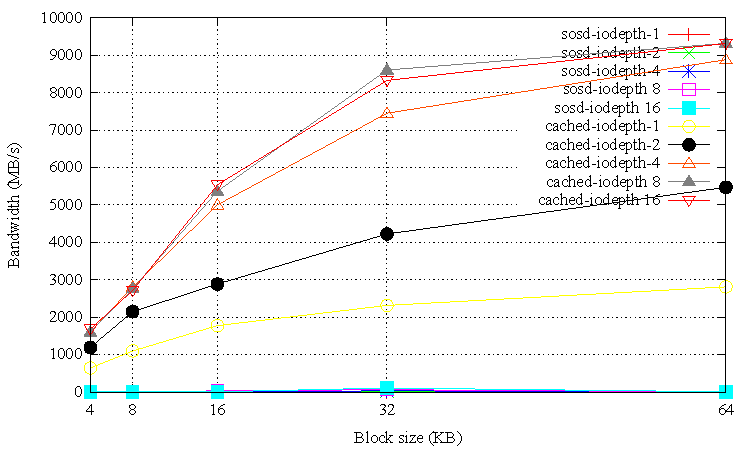
\includegraphics[]{diagrams/out.pdf}
	\caption{Cached vs. sosd}
	\label{fig:comp}
\end{figure}


Amazing results, right?

Let's see now the ugly truth...


